In recent years, the great demand for Internet services (e.g. video streaming, VoIP, etc.) has led to the exponential growth in the traffic. Therefore, having a better knowledge of the network traffic or even having a future traffic prediction becomes a critically important factor which allows network operators to efficiently perform management tasks such as traffic engineering, capacity planning and quality of service provisioning. For example, the Network Utility Maximization (NUM) \cite{ref:xu2018experience}, \cite{ref:low1999optimization} has been well studied, which usually provides a bandwidth allocation or smart routing solution by solving the optimization problem. However, these methods may suffer from an assumption that the key factors (user demands, link usages, end-to-end latency…) are given as input. These important factors are usually in the form of a traffic matrix (TM), which represents the traffic volume or latency between the origins (i.e. sources) and destinations in the network. Due to the explosion in the network traffic and the complicated, dynamic of network communication behavior, modeling and estimating the future traffic matrix have become a significant challenge. In the traditional approaches, the historical traffic data are used as the input of the regression techniques such as Autoregressive Integrated Moving Average (ARIMA) \cite{ref:box2015time} for obtaining the predicted value. However, ARIMA has a poor performance in traffic prediction due to suffering two main reasons: 1) The communication behavior has become too dynamic and complicated to model by a linear system. 2) These methods usually consider the temporal features of the traffic flow and process them independently. However, the recent studies have shown that there is a strong relation between the communication flows in the network which can be used to improve the prediction accuracy \cite{ref:wang2017spatiotemporal}.

In the last decade, deep learning has been widely applied to various application domains such as image/video processing, natural language recognition, etc. and achieved breakthrough results. In traffic analysis domain, deep learning algorithms have shown superior capability in solving the modeling and predicting non-linear time series problems. Nie et al. \cite{ref:nie2016traffic} used Restricted Boltzmann Machine to accurately predict the future traffic volume. Alternatively, the studies in \cite{ref:wang2017spatiotemporal} and \cite{ref:cao2018interactive} exploited the Convolutional Neural Network (CNN) and Long Short-Term Memory (LSTM) for capturing the spatial and temporal features and predicting the network traffic in data centers and cellular networks. Unfortunately, all of the existing algorithms proposed so far require the precise historical data as the input of the deep learning model. In the studies \cite{ref:cao2018interactive} and \cite{ref:wang2017spatiotemporal}, this requirement can easily be accomplished since the traffic in data center or cellular network is controlled through a top-of-rack switch or a base station, respectively. In contrast, collecting all the traffic data in backbone network is impractical due to the complicated network topography, resource limitation and the overhead of monitoring high speed network. Therefore, estimating the future traffic matrix in backbone network suffer from the problem of missing ground-truth input where there are some traffic flows cannot be monitored at a particular of time. A common approach to fill into the missing data is by using the data generated by the prediction model, however, this will make a huge degradation in the prediction’s performance. 

In this paper, we address the problem of modeling and predicting the future network traffic under the lack of precise historical traffic data. We leverage the combination of CNN and LSTM network which is called Convolutional LSTM network \cite{ref:xingjian2015convolutional} in extracting and modeling the spatiotemporal feature of the traffic matrix data. Besides that, the prediction accuracy of the model strongly depends on the preciseness of feeding data, the most challenging problem is how to correct the feeding data so as to minimize the gap between the feeding data and the ground-truth. To this end, we propose two techniques. First, by constructing a backward network which process the input in the inverse order of time, we have more information to correct the previous predicted data (which is always imprecise) before feeding it into the model to predict the future traffic. Secondly, we construct a mechanism to sample the ground-truth at a certain rate. Specifically, by comparing the trend and the error in the historical prediction of each flow, we design a formula to determine which flows should be monitored at the next timestep. By doing this, we can balance between the monitoring overhead (in term of flow monitored rate) and the prediction accuracy. The contribution of this paper can be summarized as follows:
\begin{itemize}
\item To our best knowledge, we are the first one considering imprecise data in the input fed to deep learning model for predicting future traffic in backbone network. Our approach is different from existing deep learning approaches in time series prediction where the model is fed with the ground-truth input.
\item We construct a model which combines the forward and backward neural network models. This model is able to correct the input data to improve the accuracy of the future prediction. Moreover, we also design a formula to determine which flows should be measured in the future.
\item We evaluate the performance of our proposed algorithms by conducting preliminary experiments on real backbone network traffic and compare the results with state-of-the-art approaches.
\end{itemize}
The rest of the paper is organized as follows: we first introduce the problem of traffic prediction under the lack of precise input data in Section 2. Section 3 presents the motivation and the details of our proposed algorithms for correcting the input data and determining the monitored flow set. Section 4 shows a preliminary experiment result and Section 5 concludes the paper.
% \begin{figure} [bt]
% \centering
% 	\subfigure[Local minimum problem.\label{fig:intro_1}]{
% 	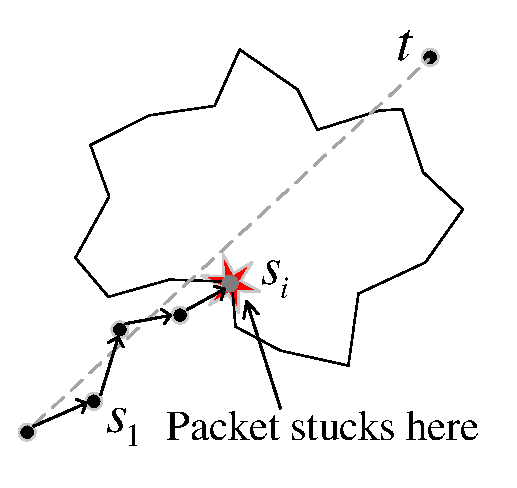
\includegraphics[width=0.35\columnwidth]{./intro_figs/intro_1.eps}
% 	}
% 	\hfill
% 	\subfigure[Congestion around the hole boundary.\label{fig:intro_2}]{
% 	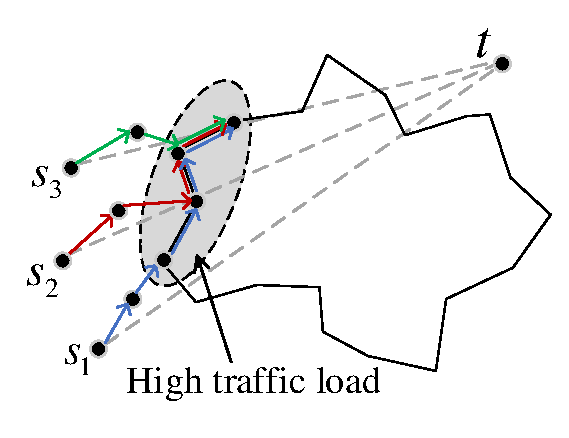
\includegraphics[width=0.4\columnwidth]{./intro_figs/intro_2.eps}
% 	}
% 	\caption{Illustrations of two serious problems that the existing protocols may encounter.}
% 	\label{fig:intro}
% \end{figure}
%
%\begin{figure*}[bt]
%    \centering
%    \begin{subfigure}[t]{0.45\textwidth}
%        \centering
%        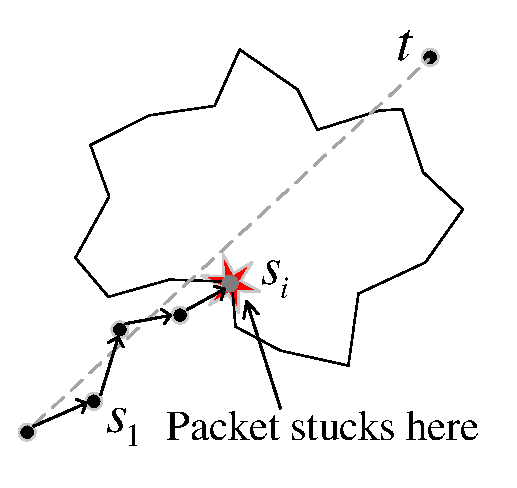
\includegraphics[width=1\columnwidth]{./intro_figs/intro_1.eps}
%        \caption{Local minimum phenomenon where the packets are stopped at the hole boundary.}
%    \end{subfigure}
%    \begin{subfigure}[t]{0.45\textwidth}
%        \centering
%        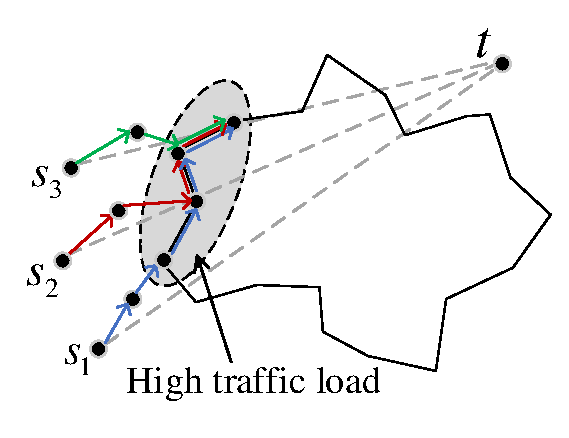
\includegraphics[width=1\columnwidth]{./intro_figs/intro_2.eps}
%        \caption{The nodes surrounding the hole boundary are imposed a heavy traffic load.}
%    \end{subfigure}
%    \caption{Illustration of two serious problems that the existing protocols may encounter.}
%\end{figure*}